The Thomas Jefferson National Accelerator Facility, also called Jefferson Lab (JLab), is one of the 17 National Laboratories in the United States \parencite{DepartmentofEnergy2023DepartmentLaboratories}, and functions mainly to deliver high energy, continuous wave (CW) electron beams to fixed-target nuclear and particle physics experiments. The facility was established in 1984 - initially named the Continuous Electron Beam Accelerator Facility (CEBAF) - and first delivered a 4 GeV electron beam on July 1 1994 to one of its three original detector halls. In 2006 efforts began to upgrade the facility to produce an electron beam up to 12 GeV in energy, which was first successfully delivered in 2015, as well as to construct a fourth detector hall for additional physics experiments\parencite{JeffersonLab2023AboutLab}. JLab is also home to a free-electron laser, capable of 10+ kW CW operation \parencite{Benson2007HighAccelerator}. 

\begin{figure}[ht]
    \centering
    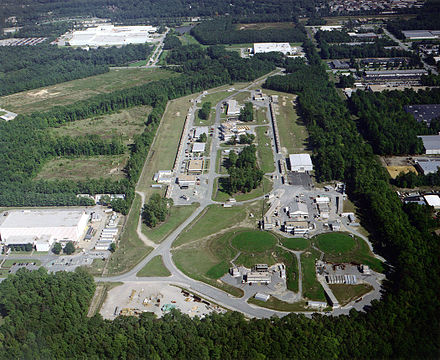
\includegraphics[width=0.8\textwidth]{Chapters/Ch2-Experiment/accel_and_beamline/pics/CEBAF/jlab_wiki.png}
    \caption{An aerial view of the Thomas Jefferson National Accelerator Facility \parencite{Wang2010CEBAFOverview}. Note that this picture was taken before the addition of the fourth detector hall (Hall D).}
    \label{fig:jlab_wiki}
\end{figure}

\subsection{Accelerator Facility}
    
    \figref{fig:jlab_accelerator_layout} shows the overarching scheme of the entire accelerator facility relevant for this experiment. Electrons are produced via the photoelectric effect from a 499 MHz pulsed laser impinges on a Gallium Arsenide photocathode (\figref{fig:gun}). The CEBAF guns operate at 100 kV and accelerate the electrons through a beam chopper (\figref{fig:chopper}) to create the desired beam structure (\figref{fig:structure}) and into the main accelerator circuit, where 1497 MHz superconducting resonator (SRF) cavities provide further acceleration (\figref{fig:klystron}). CEBAF's two $\sim$ 1.1 GV linacs accelerate electrons by consist of 50 cryomodules total, with each cryomodule housing 8 7-cell SRF cavities and the liquid helium necessary to cool them, made possible by JLab's 2K liquid helium refrigerator, the largest in the world as of 2023. The electrons are steered around the curved parts of the track by dipole magnets (\figref{fig:magnets}), making five complete circulations before delivery to the three western experimental halls.
    
    
    \begin{figure}[ht]
        \centering
        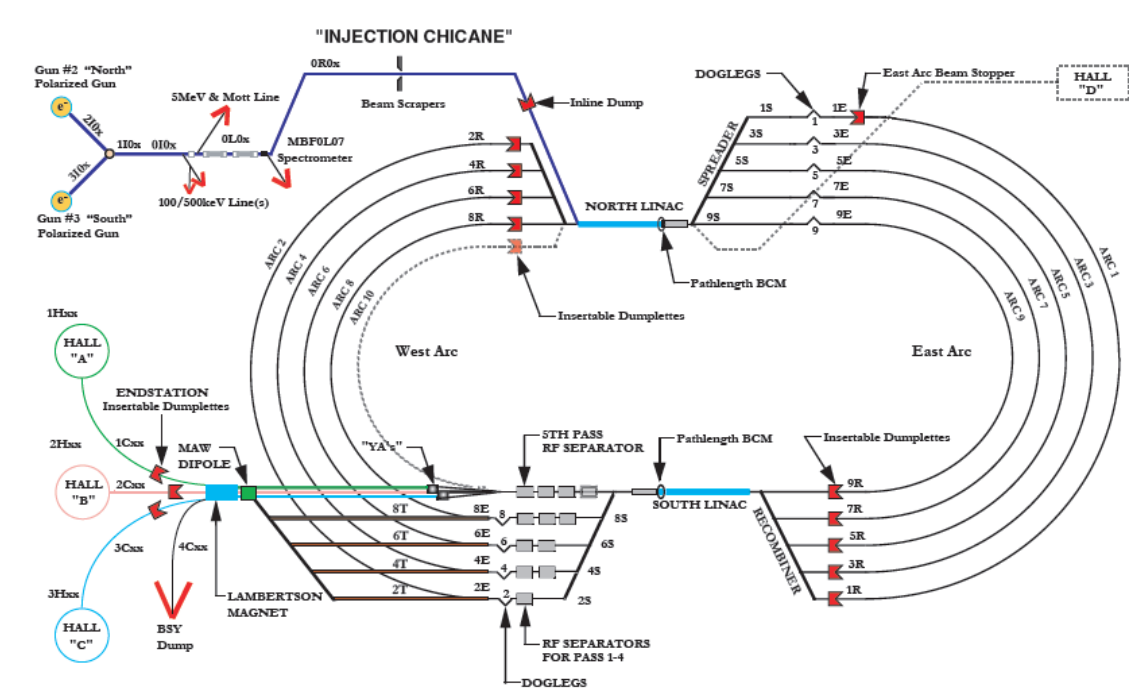
\includegraphics[width=0.8\textwidth]{Chapters/Ch2-Experiment/accel_and_beamline/pics/CEBAF/jlab-accelerator-layout.png}
        \caption{Schematic layout of the CEBAF accelerator at JLab. The racetrack configuration has two linear accelerator portions $\sim$ 1/4 mile long, and is $\sim$ 7/8 mile around \parencite{Wang2010CEBAFOverview}.}
        \label{fig:jlab_accelerator_layout}
    \end{figure}
    
    
    \begin{figure}[htb]
        \begin{minipage}[c]{\linewidth}
            \centering
            \subfloat[]{\label{fig:gun}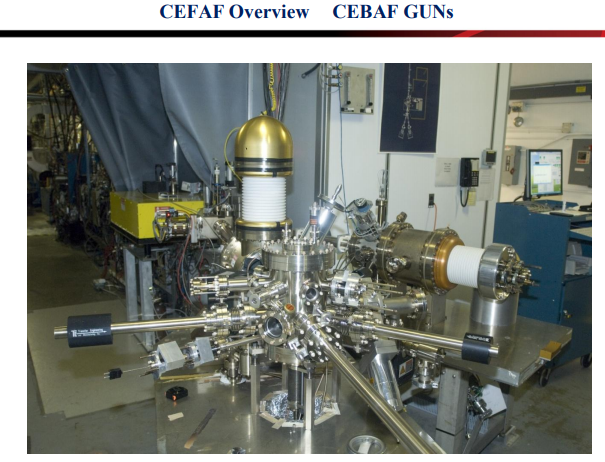
\includegraphics[width=0.3\textwidth]{Chapters/Ch2-Experiment/accel_and_beamline/pics/CEBAF/1_CEBAF-guns.png}}
            \subfloat[]{\label{fig:chopper}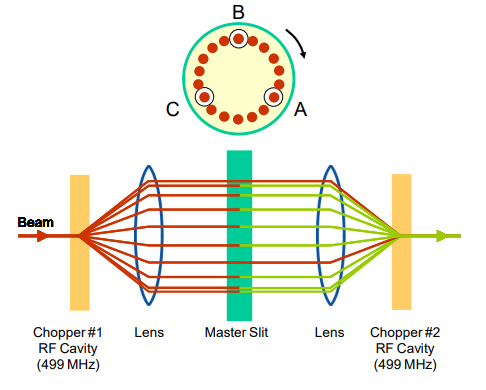
\includegraphics[width=0.3\textwidth]{Chapters/Ch2-Experiment/accel_and_beamline/pics/CEBAF/jlab-chopper.png}}
            \subfloat[]{\label{fig:structure}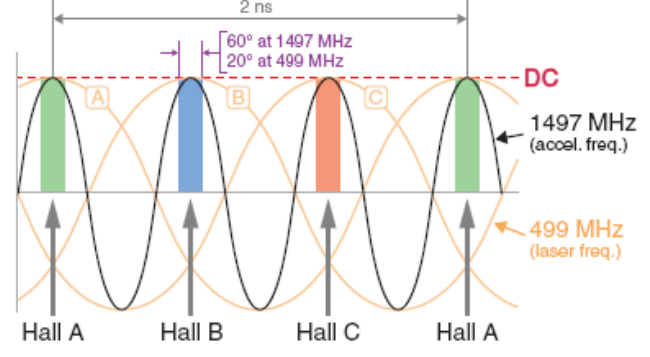
\includegraphics[width=0.3\textwidth]{Chapters/Ch2-Experiment/accel_and_beamline/pics/CEBAF/Jlab-beam-structure.png}}
        \end{minipage}
        \begin{minipage}[c]{\linewidth}
            \centering
            \subfloat[]{\label{fig:klystron}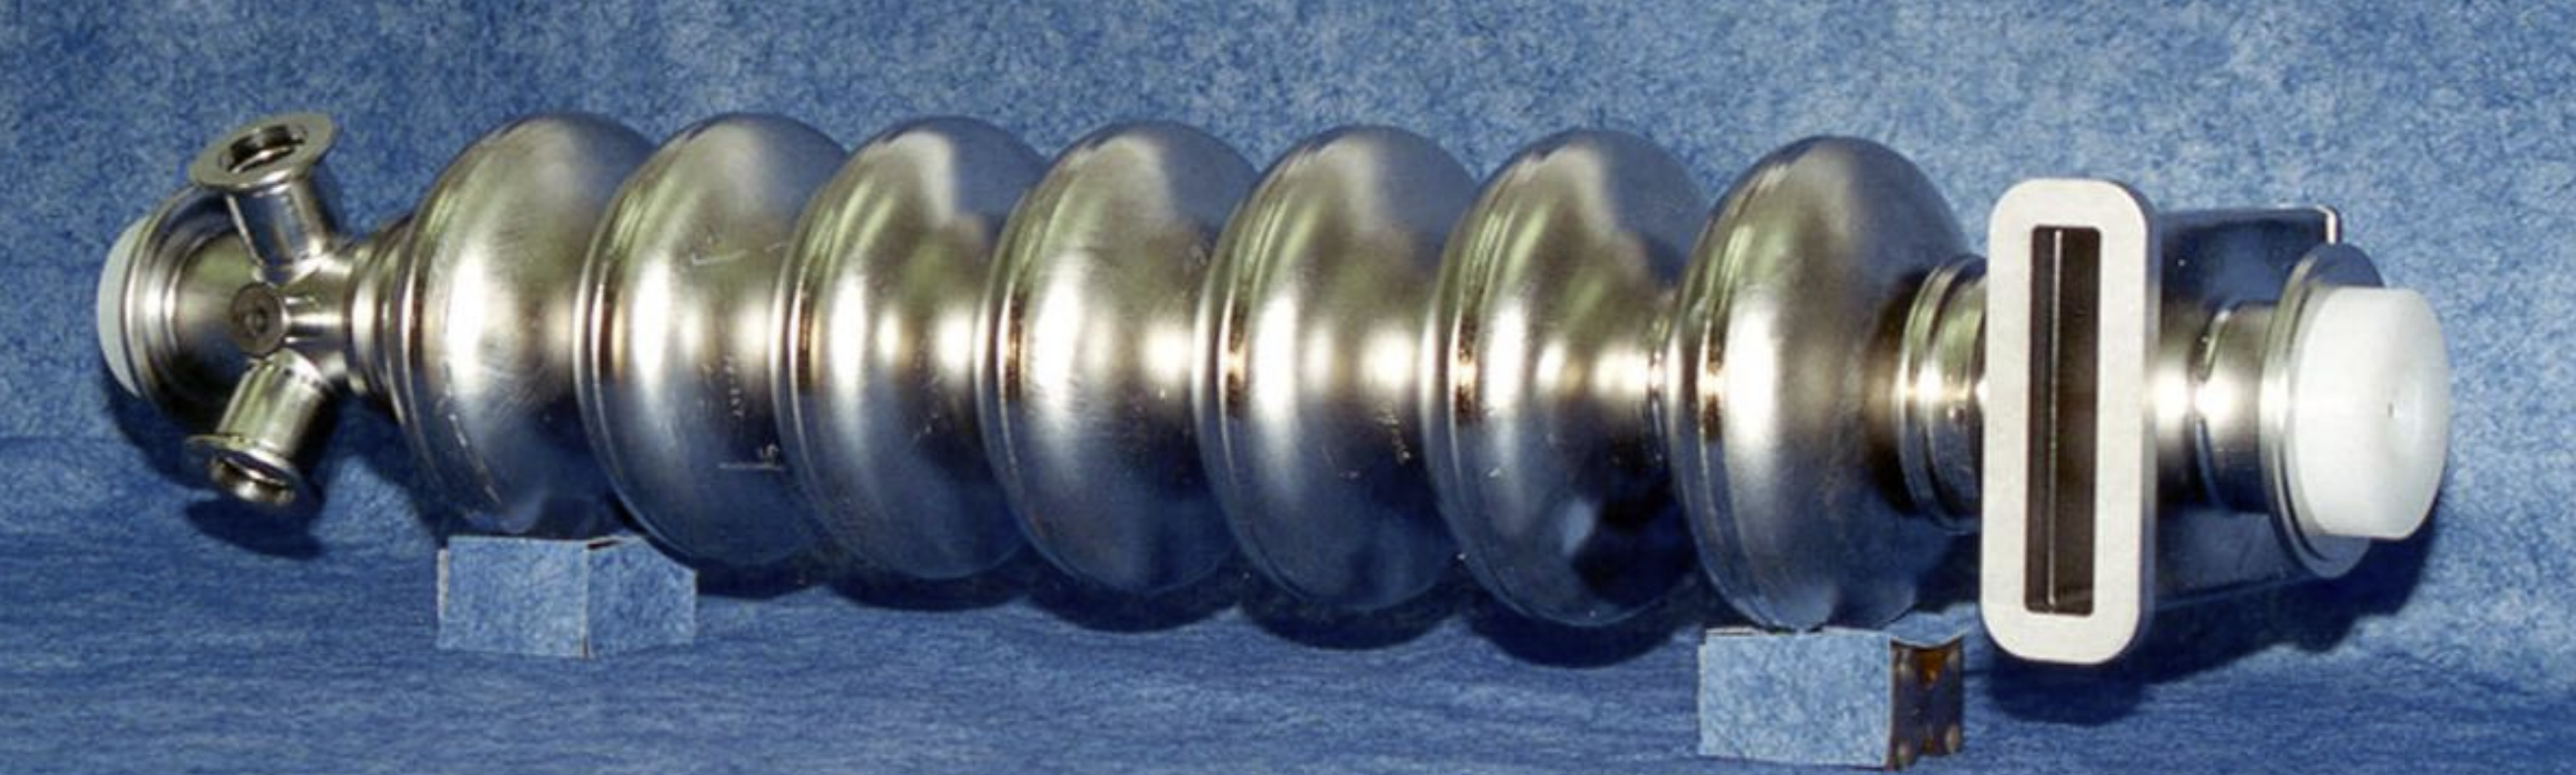
\includegraphics[width=0.4\textwidth]{Chapters/Ch2-Experiment/accel_and_beamline/pics/CEBAF/klystron.png}}
            \subfloat[]{\label{fig:magnets}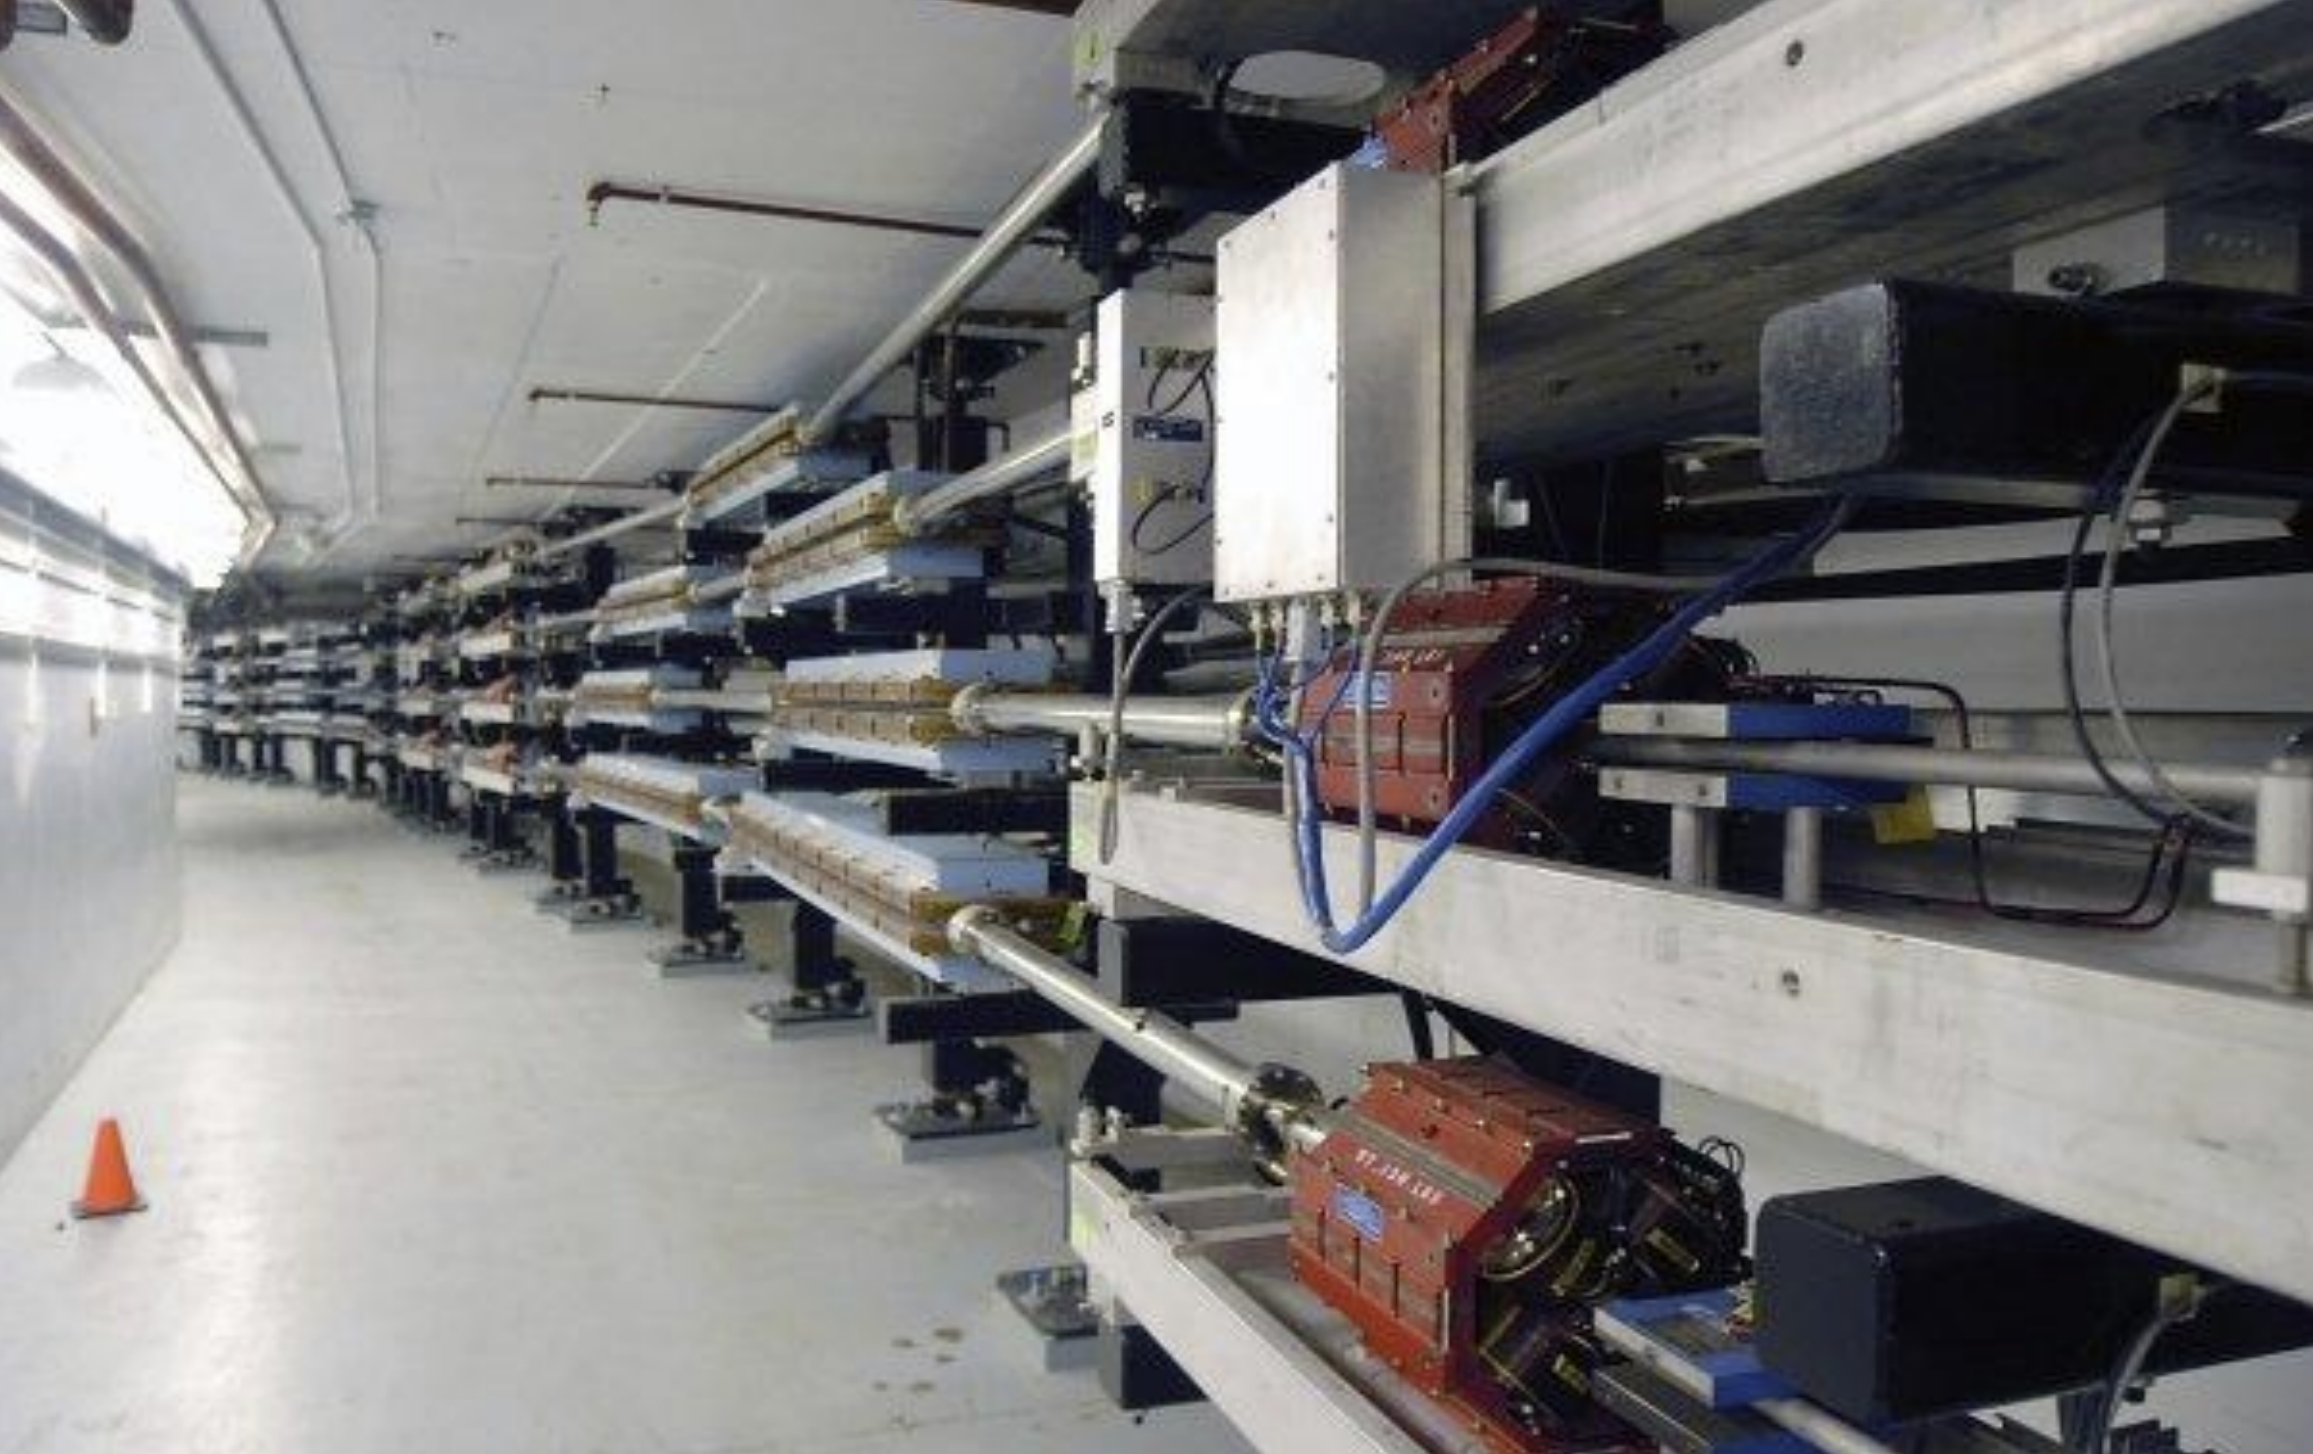
\includegraphics[width=0.4\textwidth]{Chapters/Ch2-Experiment/accel_and_beamline/pics/CEBAF/magnets2.png}}
        \end{minipage}
        \caption{(a) CEBAF guns, (b) Beam chopper, (c) Beam structure, (d) Superconducting resonator, (e) Dipole magnets.}
        \label{fig:JLab}
    \end{figure}
    

\subsection{Hall B Beamline}

    Moller polarimeters
    raster and target
    faraday cup / beamdump

    
    Finally, excess beam is safely managed using beam dumps. 
    
    \begin{figure}[ht]
        \centering
        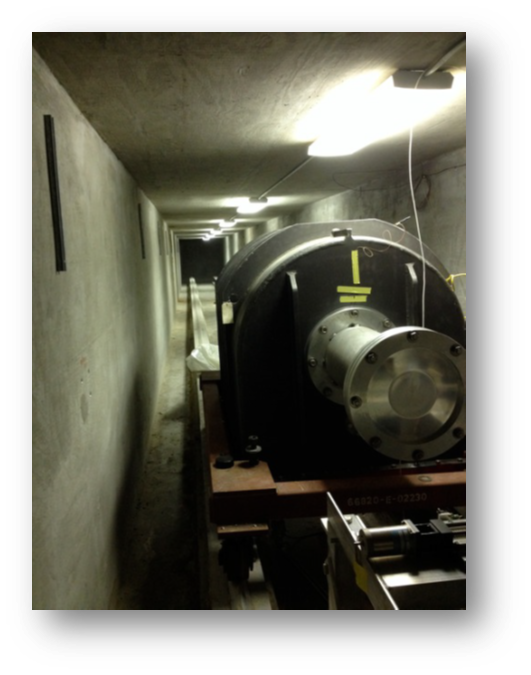
\includegraphics[width=0.8\textwidth]{Chapters/Ch2-Experiment/accel_and_beamline/pics/hallB/beamdump1.png}
        \caption{The first stage of the beam dump system at JLab.}
        \label{fig:beam_dump1}
    \end{figure}
    
    \begin{figure}[ht]
        \centering
        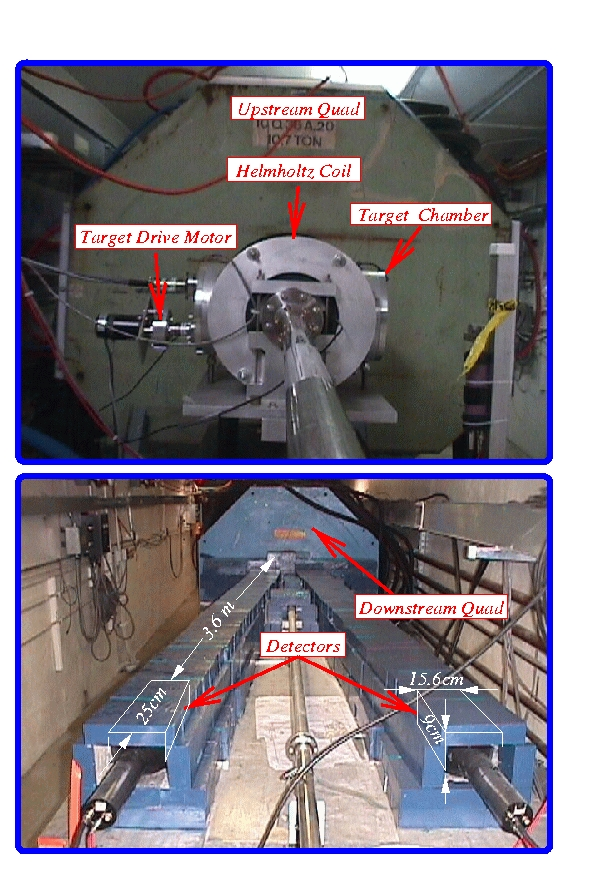
\includegraphics[width=0.8\textwidth]{Chapters/Ch2-Experiment/accel_and_beamline/pics/hallB/hall-b-poll-2.jpg}
        \caption{Moller polarimeters}
        \label{fig:beam_dump1}
    \end{figure}

    
    \begin{figure}[ht]
        \centering
        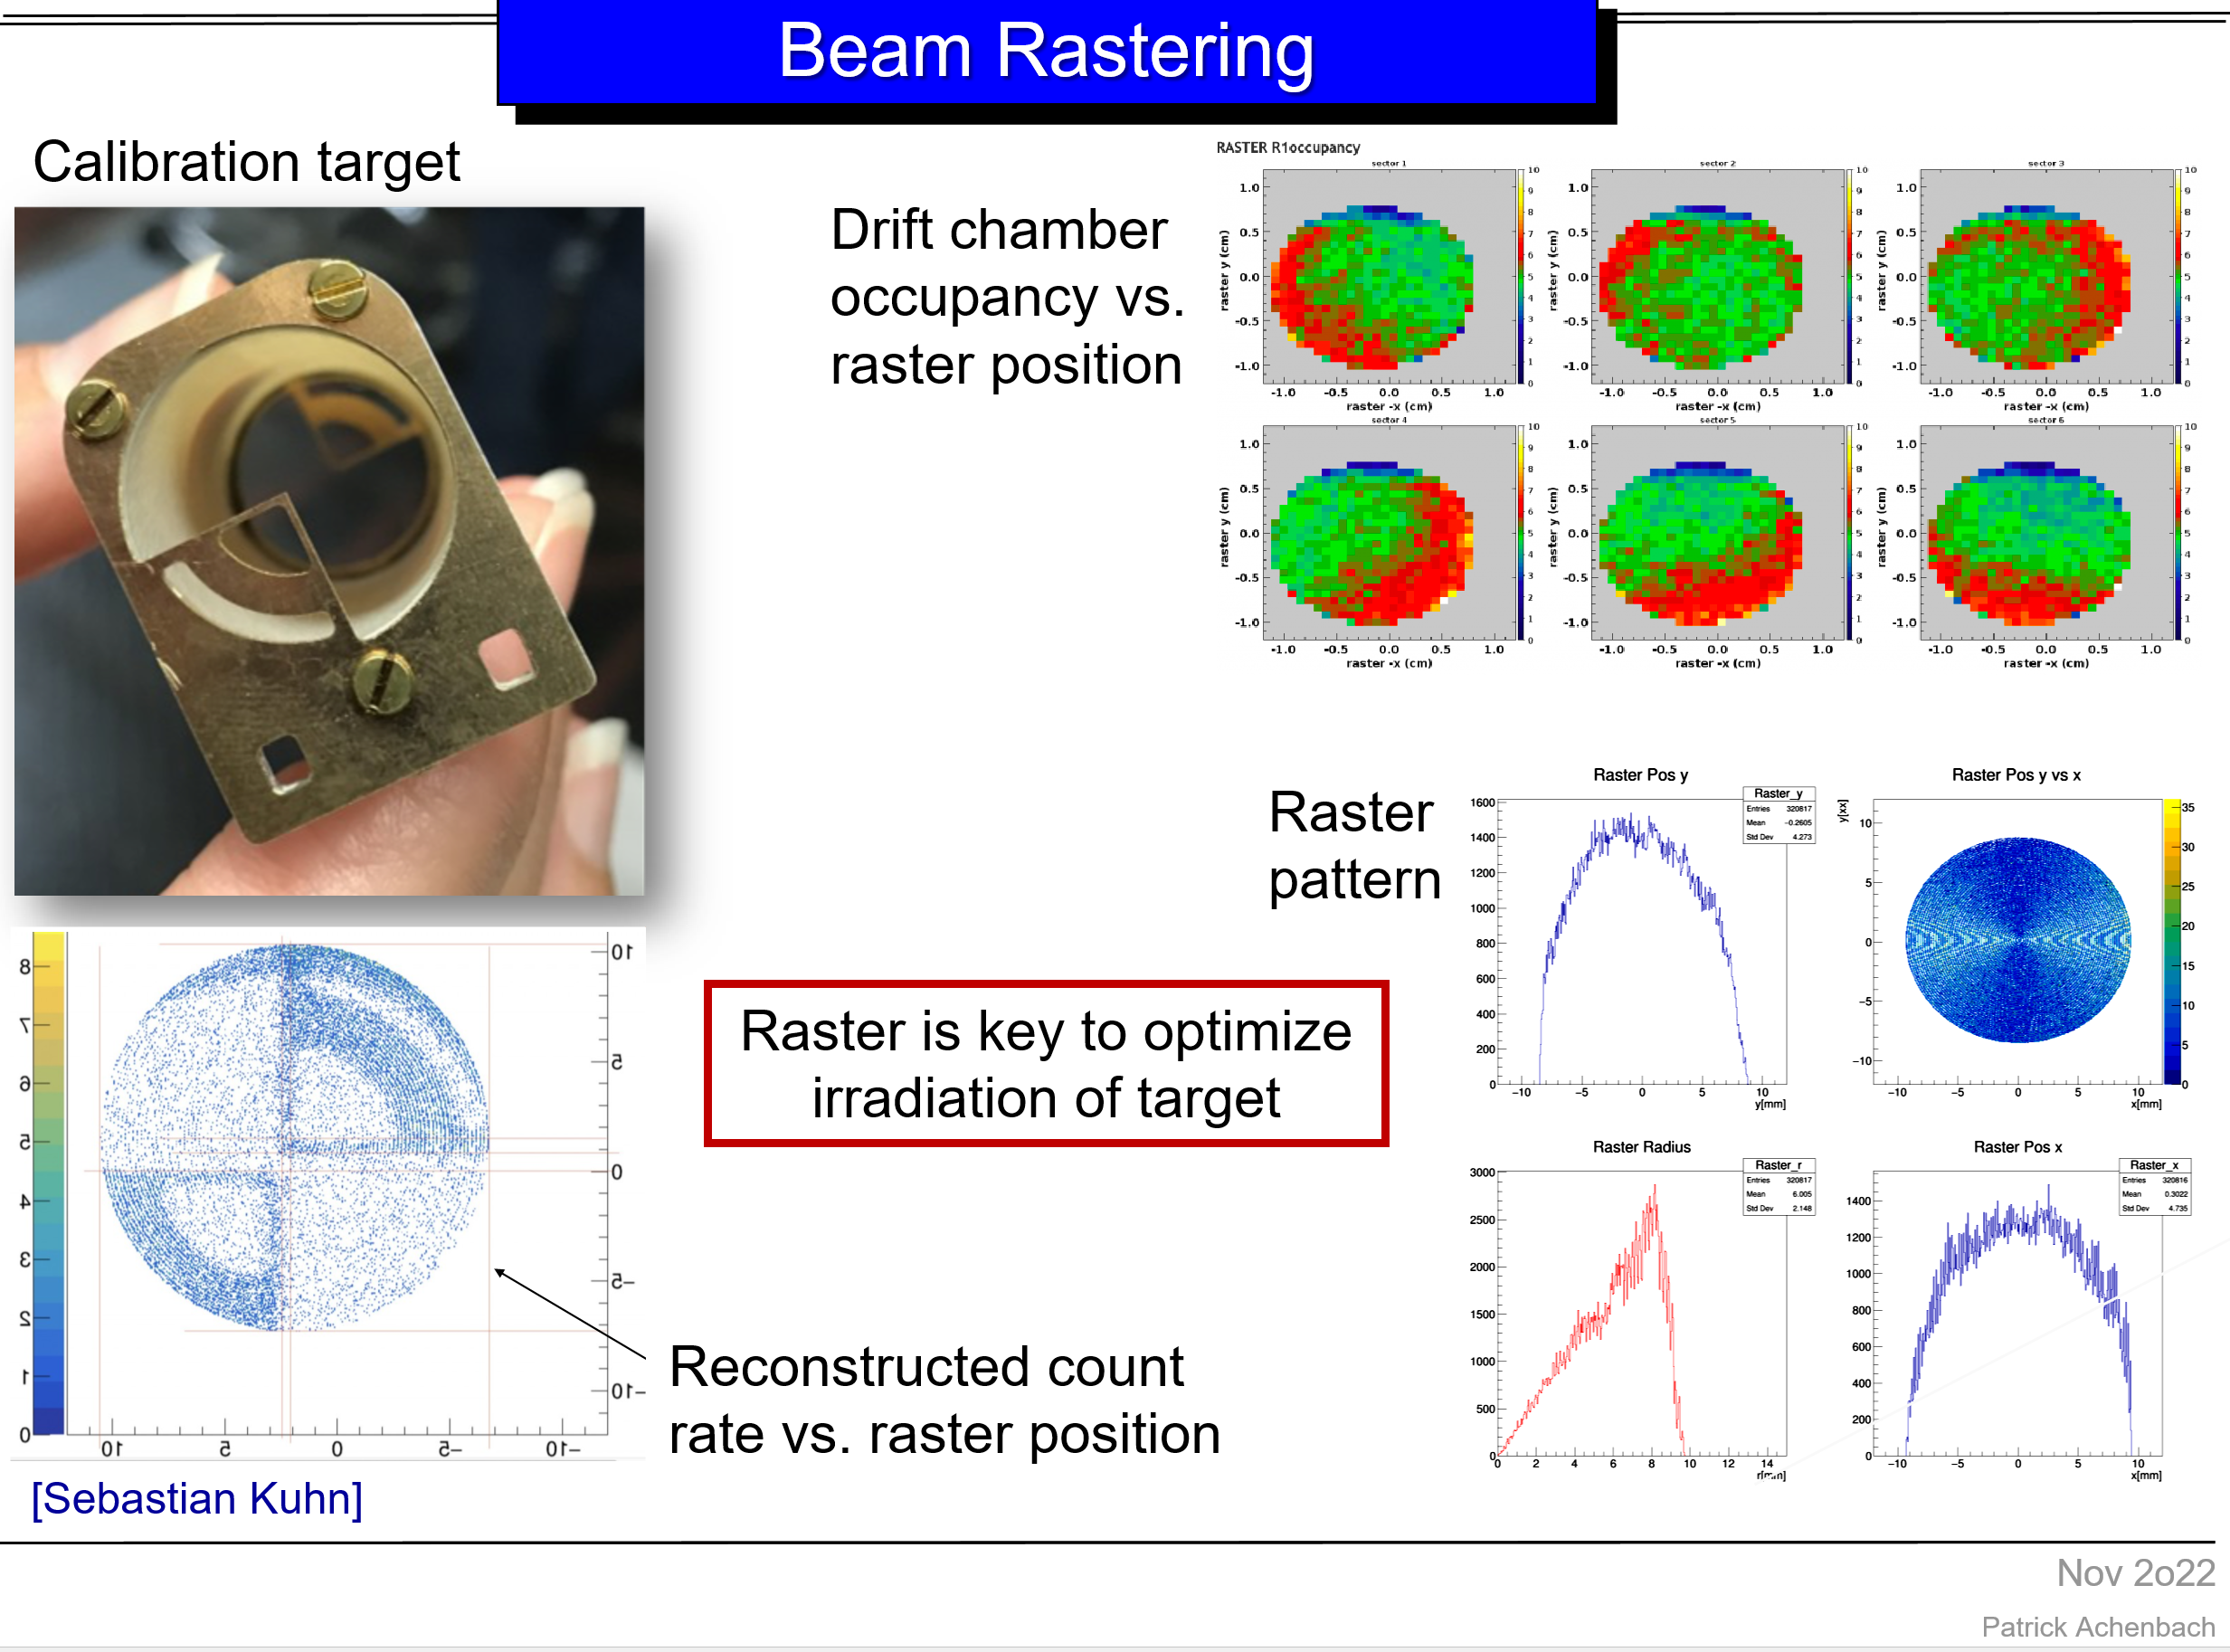
\includegraphics[width=0.8\textwidth]{Chapters/Ch2-Experiment/accel_and_beamline/pics/hallB/beam_rastering.png}
        \caption{The second stage of the beam dump system at JLab.}
        \label{fig:rastering}
    \end{figure}
    
    
    
        in beam dump area, link to own fraday cup paper \cite{Johnston2019RealizationElectrons}
        
    
    For entry into CLAS12, the beamline specs are as follows:\\
                        Beam current: up to 50 nA\\
                        Beam energy spread: $10^-4$\\
                        Beam size: Less than 0.4 mm\\
                        Beam stability: Less than 0.1 mm\\
                        Beam halo: $10^-4$\\
                        Beam polarization: up to 85\%\\
                        
    
    
    
    
    
     As stated, for RGA, the fact that the beam is polarized is not useful, but it is true and is measured by Moller Polarimeters. 
            
                Polarimietry: 
                        Good for beam energies between 100 MeV and 50 GeV. Polarized beam electrons are scat-
                tered from other polarized electrons in a target, usually magnetized foils. Only a small
                fraction of all the target electrons are polarized, so this method has a small analyzing
                power. Analyzing power is exactly calculable in QED. At high beam energies, analyzing
                power and scattering probability both become independently of beam energy. Maximum
                analyzing power is about 80%, maximum is at 90 degrees scattering angle in C.o.M. Trans-
                versely polarized target can be used to measure transverse beam polarization, but analyzing
                power is only about 10%. 90 degrees C.o.M. translates to a small lab angle with each elec-
                tron at half beam energy, so magnets are used to bend these electrons out to detectors.
                These detectors can be, for example lead glass total absorption cherenkov counters.Since
                the two electrons are corellated, can use things like time coincidence to reduce background,
                although for low duty factor accelerators only one electron is required as statistics would
                otherwise be too low.A main background to this process is Mott scattering with the electron
                radiating off energy after scattering, appearing as a Moller electron
                
                The scattering target is either iron or vanadium permendur (iron-cobalt alloy). Only 2 of
                26 electrons in iron have their spins oriented, leading to a total analyzing power of only 6 percent
                and transverse analyzing power of only 1%. Uncertainties in how magnetized the targets
                actually are corresponds to an uncertainty in analyzing power. There are ’easy’ and ’hard’
                magnetization schemes - easy does a soft magnetization, while hard uses a several tesla mag-
                net to saturate the target. In principle, uncertainties on magnetization in the hard scheme
                can be removed by using the Kerr magneto-optic effect, but this has not ever been imple-
                mented. An important correction is due to the Levchuk effect, where due to momentum
                differences between electrons in different shells, electrons scattered off of polarized electrons
                are more likely to be detected than off of unpolarized electrons. Specifically, inner electrons
                are unpolarized and have a large average momenta, so when struck they can fall outside the
                113 TOC
                acceptance of the Moller detectors, while the outer electrons, which are polarized, have a
                small average momentum, and behave as expected. This is up to a 15% effect on polarization
                measurements, and is currently a work in progress.
    
    
                
    
                 Rasterization of some kind
                    \\
                    \indent The hydrogen target in RGA is cooled to 20 K using a He4 evaporation fridge. Can by polarized by dynamic nuclear polarization, driven by a 140 GHz microwave source, can reach 90\% polarization for protons, 40\% for deuterons (both longitudinally polarized). The polarization can be measured by a Q-meter based NMR. 2.5 cm diameter target, extended 5 cm long. \\
                    \indent RGA does not use a polarized target. The beam is polarized, but the target is not, so polarization is not helpful for extracting the 5-fold differential cross section (but it would be if the target was also polarized, and is useful for BSA measurements).
                
       
                Luminosity in CLAS12 is measured from the Faraday Cup and using reference reactions such as elastic scattering. We don't use the Faraday Cup event by event, but we do use it run by run. For beam current measurements, beam position monitors upstream are used - but this is for monitoring on-line, not for analysis.
                           Can manage 175 Watts - 17 nA at 10 GeV. Is used to calibrate beam current, needs a blocker in at higher currents

\cleardoublepage
                           